{\textbf{1. 赫夫曼树}}

{{赫夫曼树又称最优二叉树,是一种带权路径长度最短的二叉树}。所谓树的带权路径长度,就是树中所有的叶结点的权值乘上其到根结点的路径长度(路径长度即路径上的分支数)。树的带权路径长度记为:}

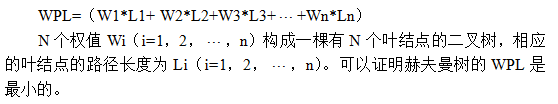
\includegraphics[width=3.70833in,height=0.68750in]{png-jpeg-pics/55D22CD2B0D12A01E2475DA33D5F35E2.png}

{\textbf{2. 构造赫夫曼树的方法}}

{{第一步:}将给定的n个权值分别看成只有根的n棵二叉树,这些二叉树构成的集合记为F。}

{{第二步:}从F中选出两棵根结点的权值最小的树(假设a和b)作为左右子树构造一棵新的二叉树(假设为c),新的二叉树的根结点的权值为左右子树根结点权值之和。}

{{第三步:}从F中删除a和b,加入c。}

{{第四步:}重复第二步和第三步,直到F中只剩下一棵树为止,这棵树便是要遍历的赫夫曼树。}

{\textbf{3. 对赫夫曼树的性质总结}}

{{性质1:}用n个权值的赫夫曼树,需要n-1次合并。}

{{性质2:}赫夫曼树中只有度为0和2的结点。}

{{性质3:}n个权值对应的赫夫曼树不唯一。}

{{性质4:}{深度为h的赫夫曼树,最大编码长度为h-1。}}

{{性质5:}{赫夫曼编码是能使电文代码总长最短的编码方式。}}

{{{性质6:}赫夫曼是一种前缀编码(就是任一字符的编码,都不是另一个字符编码的前缀)。}}

{\textbf{4. 赫夫曼编码}}

{根据给定字符值求赫夫曼编码的过程,实质就是根据给定权值构造赫夫曼树的过程。以a、b、c、d的出现频率为0.4、0.3、0.1、0.2为例,求赫夫曼编码过程如下:}

{{第一步:}根据权值构造赫夫曼树。}

{{第二步:}对构造好的赫夫曼树,约定左分支为0,右分支为1。}

{{第三步:}从根结点到叶子结点的分支上的编码组成该叶子结点的赫夫曼编码,A为0,B为10,C为110,D为111,如下图所示。}

{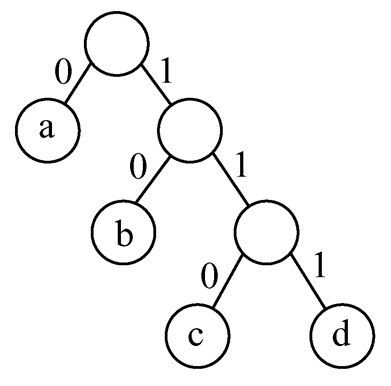
\includegraphics[width=2.08333in,height=2.08333in]{png-jpeg-pics/bb7b22b1f9410526bd709b8b58bf6702?}}
